\hypertarget{carrying-capacity}{%
\subsection{Carrying capacity}\label{carrying-capacity}}

\hypertarget{motivation}{%
\subsubsection{Motivation}\label{motivation}}

This pattern can help project participants recognize and communicate
their stresses to make themselves and the project more resilient.

\hypertarget{context}{%
\subsubsection{Context}\label{context}}

One of the important maxims from the world of FLOSS is: ``Given enough
eyeballs, all bugs are shallow'' {{[}8{]}}. A partial converse is also
true: there's only so much any one person can do, since we all have
limited time and energy.

\hypertarget{forces}{%
\subsubsection{Forces}\label{forces}}

\begin{quote}

\includegraphics{images/antifragility.png} \textbf{Antifragility}: each
person's potential can only be realized if people take on enough, but
not too much.\\

\includegraphics{images/independence.png} \textbf{Independence}: in a
peeragogy context, it is often impossible to delegate work to others.
\end{quote}

\hypertarget{problem}{%
\subsubsection{Problem}\label{problem}}

How can we help prevent those people who are involved with the project
from over-promising or over-committing, and subsequently crashing and
burning? First, let's be clear that there are lots of ways things can go
wrong. Simplistic expectations -- like \emph{assuming that others will
do the work for you} {{[}13{]}} -- can undermine your ability to
correctly gauge your own strengths, weaknesses, and commitments. Without
careful, critical engagement, you might not even notice when there's a
problem. Where one person has trouble letting go, others may have
trouble speaking up. Pressure builds when communication isn't going
well.

\hypertarget{solution}{%
\subsubsection{Solution}\label{solution}}

Serious frustration is a sign that it's time to revisit the group's and
your own individual plan. Are these realistic? If you have a ``buddy''
they can provide a reality check. Maybe things are not \emph{that hard}
after all -- and maybe they don't need to be done \emph{right now}.
Generalizing from this: the project can promote an open dialog by
creating opportunities for people to share their worries and generate an
emergent plan for addressing them {{[}10{]}}. Use the project to make
note of obstacles. For example, if you'd like to pass a baton, you'll
need someone there who can take it. Maybe you can't find that person
right away, but you can bring up the concern and get it onto the
project's . The situation is always changing, but if we continue to
create suitable checkpoints and benchmarks, then we can take steps to
take care of an issue that's getting bogged down.

\hypertarget{rationale}{%
\subsubsection{Rationale}\label{rationale}}

Think of the project as an ecosystem populated by acts of participation.
As we get to know more about ourselves and each other, we know what
sorts of things we can expect, and we are able to work together more
sustainably {{[}6{]}}. We moderate stress and improve collective
outcomes by taking concerns seriously.

\hypertarget{resolution}{%
\subsubsection{Resolution}\label{resolution}}

Guiding and rebalancing behavior in a social context can begin with
speaking up about a concern. When we acknowledge concerns, we must take
into account our own boundedness. We have find an opportunity to make
ourselves helpful, without impinging on others' \textbf{independence}.
This doesn't mean allowing all possible stresses to run rampant: we work
to stay within the realm of \textbf{antifragility}, where manageable
stress \emph{improves} the system rather than degrading it {{[}12{]}}.
As we share concerns and are met with care and practical support, our
actions begin to align better with expectations (often as a result of
forming more realistic expectations).

\hypertarget{example-1}{%
\subsubsection{Example 1}\label{example-1}}

Wikipedia aims to emphasize a neutral point of view, but its users are
not neutral.\footnote{\url{https://en.wikipedia.org/wiki/Wikipedia:Neutral_point_of_view}}
topics that matter to them.\footnote{\url{https://en.wikipedia.org/wiki/Wikipedia:Activist}}
and participation are not neutral in another less sanguine sense. More
information on Wikipedia deals with Europe than all of the locations
outside of Europe {{[}2{]}}. As we remarked in the pattern, most of the
actual work is contributed by a small percentage of users. The
technology limits the kinds of things that can be said {{[}2{]}}. The
total number of active editors has been falling since 2007.\footnote{\url{https://strategy.wikimedia.org/wiki/Editor_Trends_Study/Results}}
Some blame outmoded technology and an insider culture {{[}11{]}}, or a
stringent editorial approach that emerged in response to the site's
popularity {{[}3{]}}. Others highlight the rise of successful
competition, often inspired by wiki models, but driven by ``corporate
logic'' {{[}4,5{]}}. Some proposed solutions focus on various indicators
of ``community health.''\footnote{\url{https://lists.wikimedia.org/pipermail/wiki-research-l/2016-January/004959.html}}

\hypertarget{example-2}{%
\subsubsection{Example 2}\label{example-2}}

Progressive thinkers have for some time subscribed to the view that
``there shall be no women in case there be not men, nor men in case
there be not women'' {{[}7{]}}. A separate Ladies Hall seems entirely
archaic. However, in light of the extreme gender imbalance in free
software, and still striking imbalance at Wikipedia {{[}1,9{]}}, it will
be important to do whatever it takes to make women and girls welcome,
not least because this is a significant factor in boosting our .

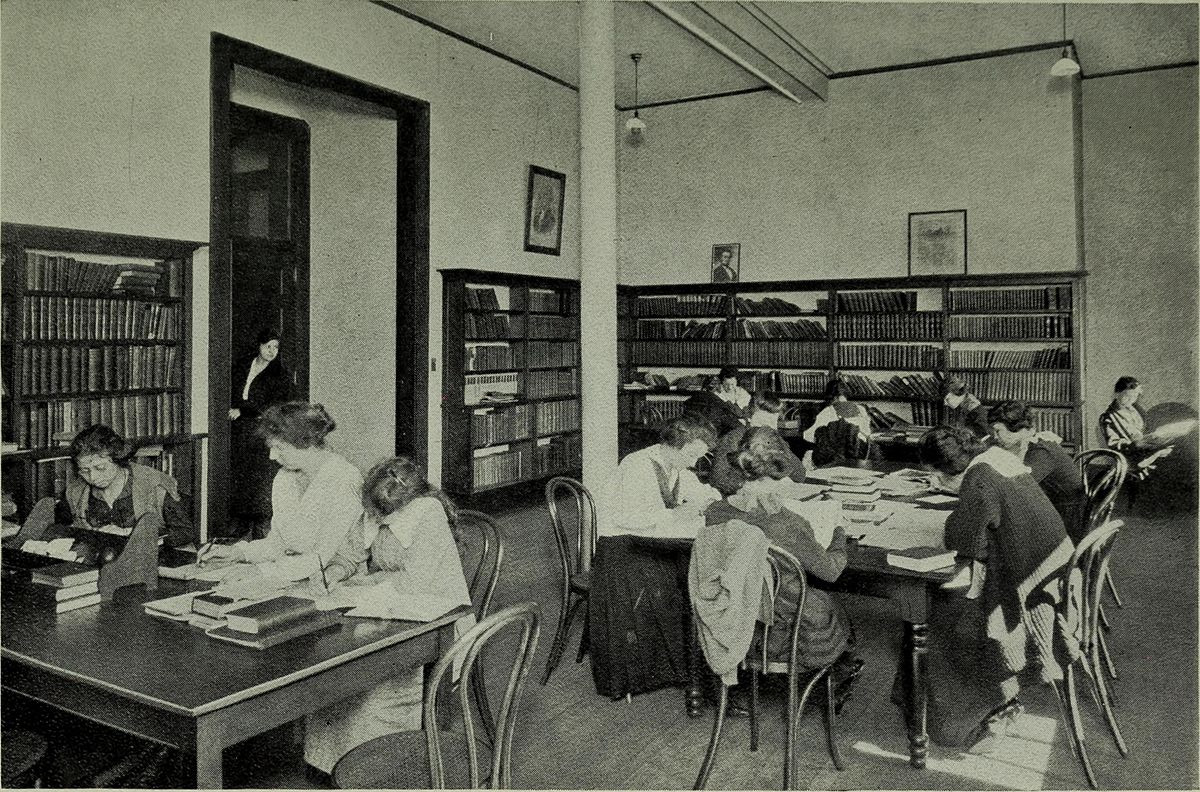
\includegraphics{images/ladies-hall.jpg}\\
\emph{Ladies Hall: Queens College, North Carolina.}

\hypertarget{whats-next-in-the-peeragogy-project}{%
\subsubsection{What's Next in the Peeragogy
Project}\label{whats-next-in-the-peeragogy-project}}

Making it easy and fruitful for others to get involved is one of the
best ways to redistribute the load. This often requires knowledge
transfer and skill development among those involved; see .

\hypertarget{references}{%
\subsubsection{References}\label{references}}

\begin{enumerate}
\def\labelenumi{\arabic{enumi}.}
\item
  Rishab A. Ghosh, Ruediger Glott, Bernhard Krieger, and Gregorio
  Robles. 2002. \emph{Free/Libre and Open Source Software: Survey and
  Study}. International Institute of Infonomics, University of
  Maastricht.
\item
  Mark Graham, Bernie Hogan, Ralph K Straumann, and Ahmed Medhat. 2014.
  Uneven geographies of user-generated information: Patterns of
  increasing informational poverty. \emph{Annals of the Association of
  American Geographers} 104, 4: 746--764.
\item
  Aaron Halfaker, R. Stuart Geiger, Jonathan Morgan, and John Riedl.
  2013. The Rise and Decline of an Open Collaboration System: How
  Wikipedia's reaction to sudden popularity is causing its decline.
  \emph{American Behavioral Scientist} 57, 5: 664--688.
  \url{http://doi.org/10.1177/0002764212469365}
\item
  Daniel Kreiss, Megan Finn, and Fred Turner. 2011. The limits of peer
  production: Some reminders from Max Weber for the network society.
  \emph{New Media \& Society} 13, 2: 243--259.
\item
  Mayo Fuster Morell. 2011. An introductory historical contextualization
  of online creation communities for the building of digital commons:
  The emergence of a free culture movement. \emph{Proceedings of the 6th
  Open Knowledge Conference}. Retrieved from
  \url{http://ceur-ws.org/Vol-739/paper_7.pdf}
\item
  Elinor Ostrom. 2010. Revising theory in light of experimental
  findings. \emph{Journal of Economic Behavior \& Organization} 73, 1:
  68--72.
\item
  François Rabelais. {[}1534{]} 1894. \emph{Gargantua and pantagruel}.
  Moray Press.
\item
  Eric S Raymond. 2001. \emph{The Cathedral \& the Bazaar: Musings on
  Linux and open source by an accidental revolutionary}. O'Reilly Media,
  Inc.
\item
  Joseph Reagle. 2012. ``Free as in sexist?'' Free culture and the
  gender gap. \emph{First Monday} 18, 1. Retrieved from
  \url{http://firstmonday.org/ojs/index.php/fm/article/view/4291}
\item
  Jaakko Seikkula and Tom Erik Arnkil. 2006. \emph{Dialogical meetings
  in social networks}. Karnac Books.
\item
  Tom Simonite. 2013. The Decline of Wikipedia. \emph{Technology Review}
  116, 6: 50--56.
\item
  Nassim Nicholas Taleb. 2012. \emph{Antifragile: Things that gain from
  disorder}. Random House Incorporated.
\item
  Linus Torvalds and Steven Vaughan-Nichols. 2011. Linus Torvalds's
  Lessons on Software Development Management. \emph{Input Output}.
  Retrieved from
  \url{http://web.archive.org/web/20131021211847/http://h30565.www3.hp.com/t5/Feature-Articles/Linus-Torvalds-s-Lessons-on-Software-Development-Management/ba-p/440}
\end{enumerate}

\begin{center}\rule{0.5\linewidth}{0.5pt}\end{center}
